% generated by experiments/make_tex_figures.py -- do not edit by hand
\begin{figure}[t]
\centering
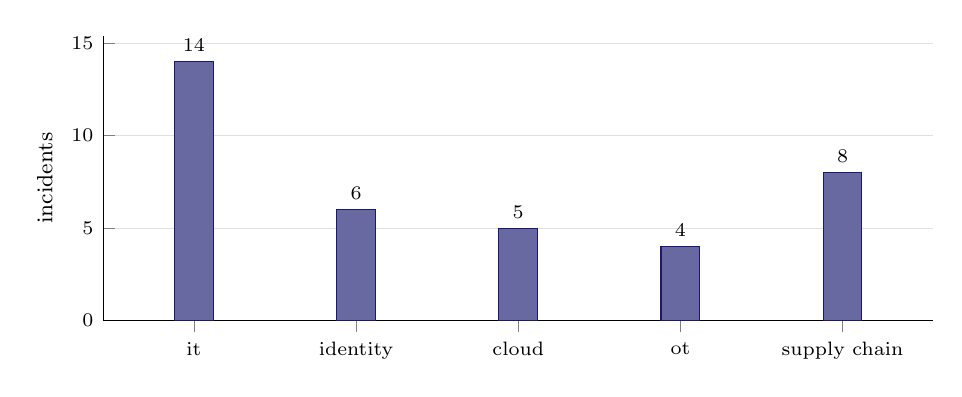
\begin{tikzpicture}
\begin{axis}[
    ybar, width=\linewidth, height=5.2cm,
    ylabel={incidents}, symbolic x coords={it,identity,cloud,ot,supply chain},
    xtick=data, ymin=0, bar width=14pt, enlarge x limits=0.14,
    nodes near coords, nodes near coords style={font=\scriptsize},
    ticklabel style={font=\scriptsize}, label style={font=\footnotesize},
    ymajorgrids, grid style={gray!25}, axis lines*=left,
]
\addplot[fill=MidnightBlue!65, draw=MidnightBlue] coordinates {(it,14) (identity,6) (cloud,5) (ot,4) (supply chain,8)};
\end{axis}
\end{tikzpicture}
\caption{Planes traversed by the 20 corpus incidents (2017--2025). Only two
incidents are reported to have interacted with equipment below Purdue level~3.}
\label{fig:corpus-planes}
\end{figure}
